\subsubsection{\cmsC{Prospects for leptoquark searches in $t$+$\tau$ and $t$+$\mu$ decays}}
\contributors{A. Reimers$^a$, R. Kogler$^a$, J. Haller$^a$, CMS}
%{\bf Author(s): A. Reimers$^a$, R. Kogler$^a$, J. Haller$^a$, CMS}
%\noindent \textit{a) Institut f\"{u}r Experimentalphysik, Universit\"{a}t Hamburg, Germany}

Leptoquarks (LQs) are hypothetical particles that carry both baryon and lepton quantum numbers. They are color-triplets and carry fractional electric charge. The spin of a LQ state is either 0 (scalar LQ) or 1 (vector LQ). At the LHC, the pair-production of LQs is possible via gluon-gluon fusion and quark-antiquark annihilation. The pair production cross section depends on the mass of the LQ. For scalar LQs, it is known at NLO in perturbative QCD~\cite{Kramer:2004df}.

The reach of searches for pair production of LQs with decays to $t+\mu$ and $t+\tau$ is studied for the HL-LHC with target integrated luminosities of 
$\mathcal{L}_{\text{int}}^{\text{target}} = 300$ and $3000\,\mathrm{fb}^{-1}$~\cite{CMS-PAS-FTR-18-008}. The studies are based on published CMS results of the $t$+$\mu$~\cite{Sirunyan:2018ruf} and $t$+$\tau$~\cite{Sirunyan:2018nkj} LQ decay channels which use data of proton-proton collisions at $\sqrt{s}=13\,\mathrm{TeV}$ corresponding to $\mathcal{L}_{\text{int}} = 35.9\,\mathrm{fb}^{-1}$ recorded in 2016. While the analysis strategies are kept unchanged with respect to the ones in \citerefs{Sirunyan:2018nkj, Sirunyan:2018ruf}, different total integrated luminosities, the higher \com energy of 14\,TeV, and different scenarios of systematic uncertainties are considered. In the first scenario (denoted ``w/ YR18 syst. uncert.''), the relative experimental systematic uncertainties are scaled by a factor of $1 / \sqrt{f}$, with 
$f=\mathcal{L}_{\text{int}}^{\text{target}}/35.9\,\mathrm{fb}^{-1}$, 
until they reach a defined lower limit based on estimates of the achievable accuracy with the upgraded detector~\cite{CMS:FTR-18-012}. The relative theoretical systematic uncertainties are halved. In the second scenario (denoted ``w/ stat. uncert. only''), no systematic uncertainties are considered. The relative statistical uncertainties in both scenarios are scaled by $1 / \sqrt{f}$.

Figure~\ref{fig:LQpairs:significances} presents the expected signal significances of the analyses as a function of the LQ mass for different assumed integrated luminosities in the ``w/ YR18 syst. uncert.'' and ``w/ stat. uncert. only'' scenarios. Increasing the target integrated luminosity to $\mathcal{L}_{\text{int}}^{\text{target}} = 3000\,\mathrm{fb}^{-1}$ greatly increases the discovery potential of both analyses. The LQ mass corresponding to a discovery at $5\sigma$ significance with a dataset corresponding to $3000\,\mathrm{fb}^{-1}$ increases by more than 500\,GeV compared to the situation at $\mathcal{L}_{\text{int}}^{\text{target}} = 35.9\,\mathrm{fb}^{-1}$, from about 1200\,GeV to roughly 1700\,GeV, in the $\text{LQ}\rightarrow t\mu$ decay channel. For LQs decaying exclusively to top quarks and $\tau$ leptons, a gain of 400\,GeV is expected, pushing the LQ mass in reach for a $5\sigma$ discovery from 800\,GeV to 1200\,GeV. 

\begin{figure}[t]
\centering
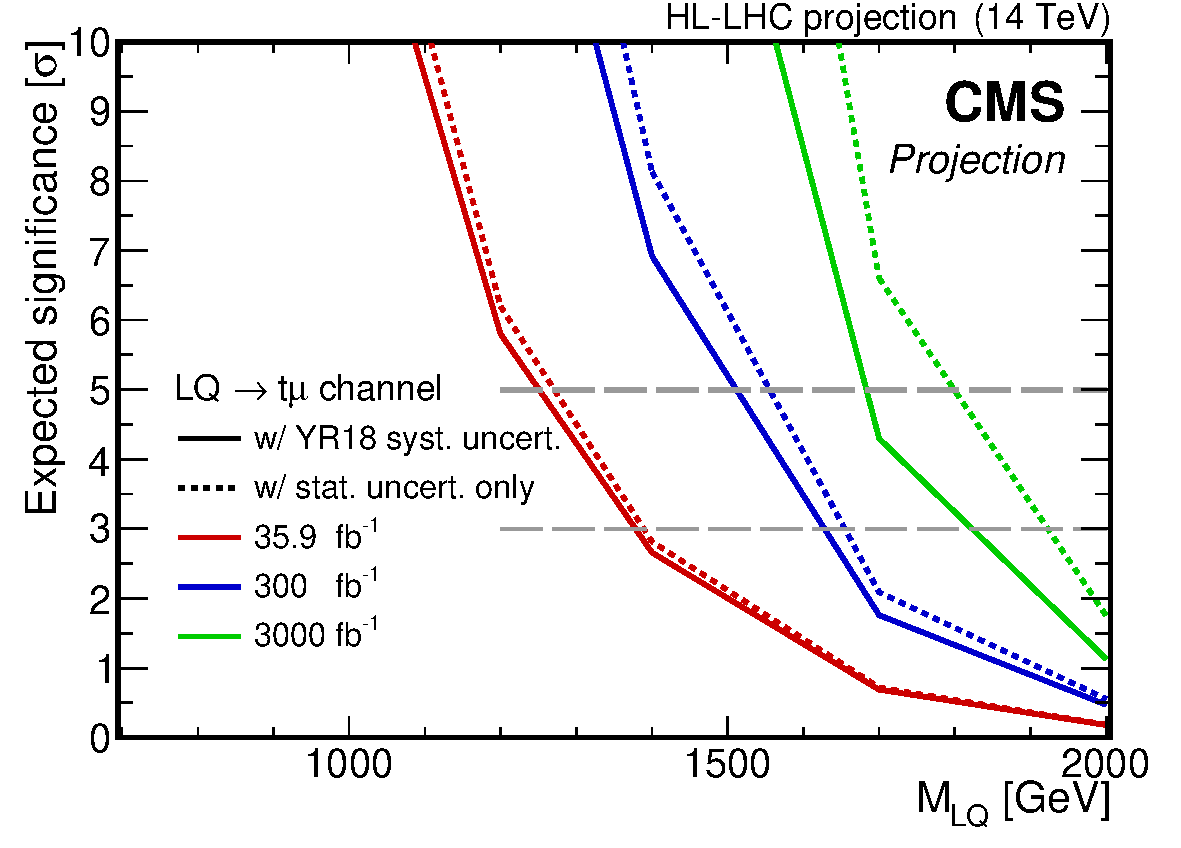
\includegraphics[width=0.49\textwidth]{\main/section7OtherSignatures/img/LQpairs_Sign_tmu.pdf}
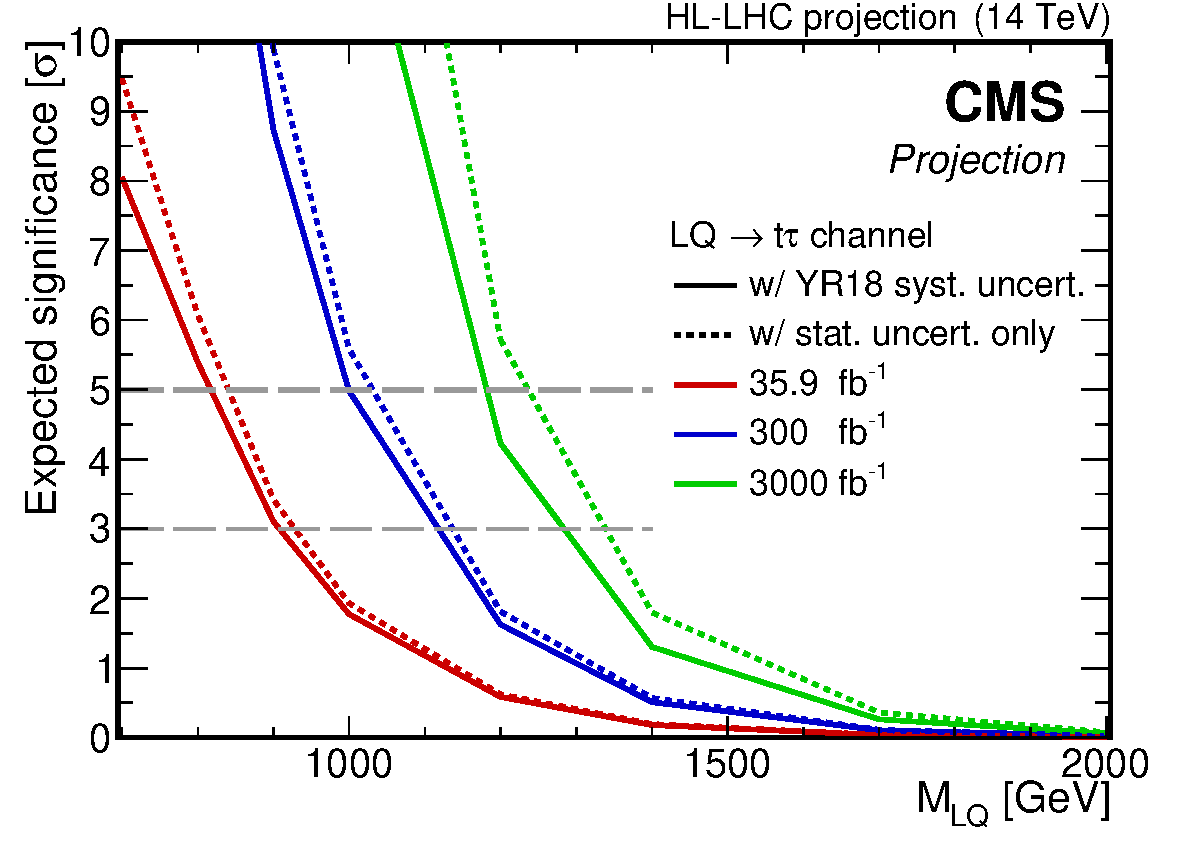
\includegraphics[width=0.49\textwidth]{\main/section7OtherSignatures/img/LQpairs_Sign_ttau.pdf}
\caption{Expected significances for an LQ decaying exclusively to top quarks and muons (left) or $\tau$ leptons (right).}
\label{fig:LQpairs:significances}
\end{figure}

In \fig{fig:LQpairs:limits1d}, the expected projected exclusion limits on the LQ pair production cross section are shown. Leptoquarks decaying only to top quarks and muons are expected to be excluded below masses of 1900\,GeV for $3000\,\mathrm{fb}^{-1}$, which is a gain of 500\,GeV compared to the limit of 1420\,GeV obtained in the published analysis of the 2016 dataset~\cite{Sirunyan:2018ruf}. The mass exclusion limit for LQs decaying exclusively to top quarks and $\tau$ leptons are expected to be increased by 500\,GeV, from 900\,GeV to approximately 1400\,GeV.

\begin{figure}[t]
\centering
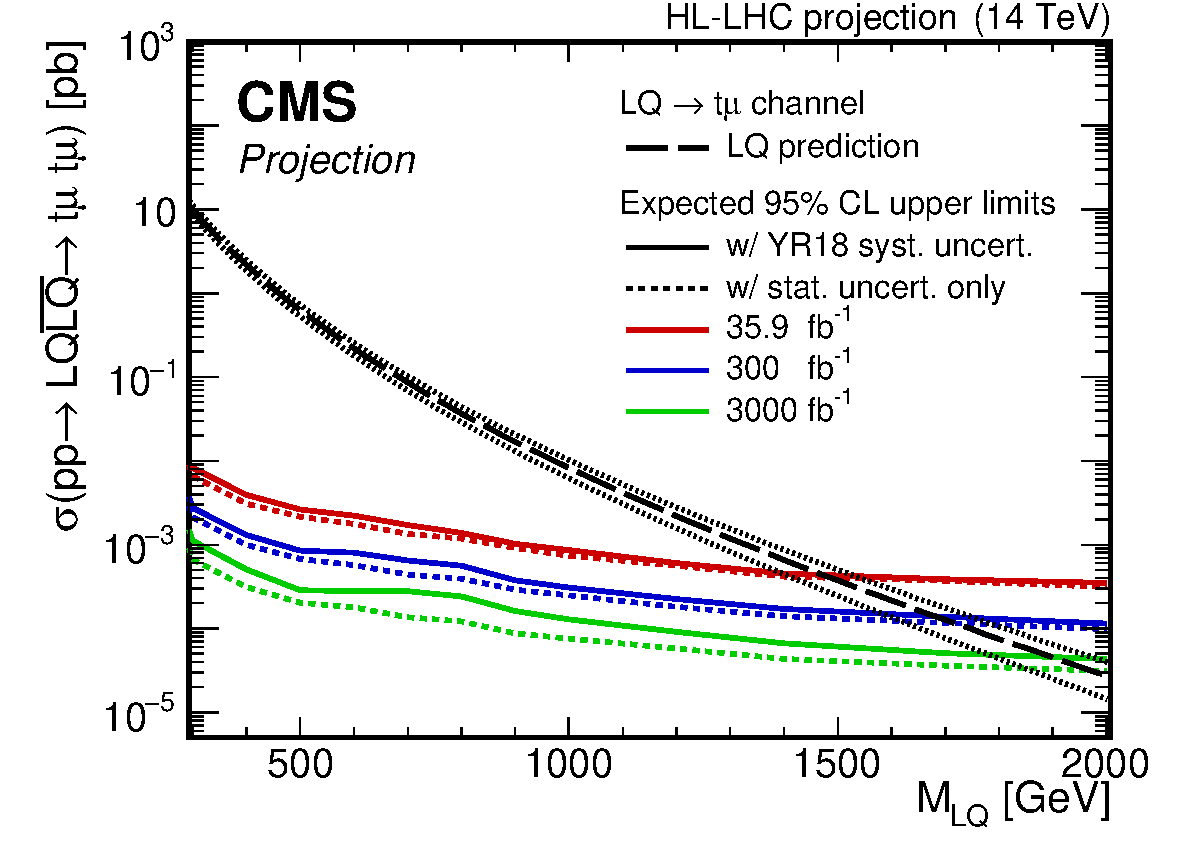
\includegraphics[width=0.49\textwidth]{\main/section7OtherSignatures/img/LQpairs_Limits_tmu.pdf}
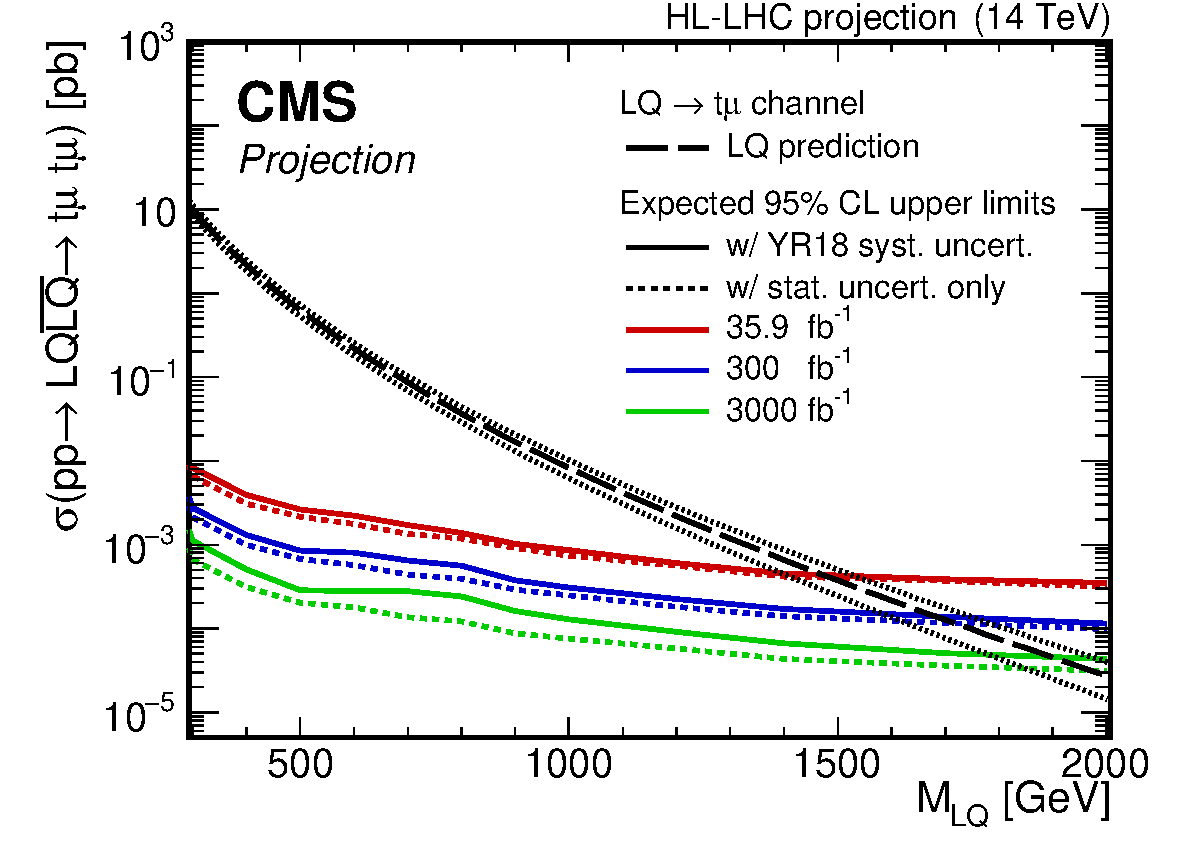
\includegraphics[width=0.49\textwidth]{\main/section7OtherSignatures/img/LQpairs_Limits_tmu.pdf}
\caption{Expected upper limits on the LQ pair production cross section at the 95\%~\cl for an LQ decaying exclusively to top quarks and muons (left) or $\tau$ leptons (right).}
\label{fig:LQpairs:limits1d}
\end{figure}

Figure~\ref{fig:LQpairs:limits2d} shows the expected signal significances and upper exclusion limits on the pair production cross section of scalar LQs allowed to decay to top quarks and muons or $\tau$ leptons at the 95\%~\cl as a function of the LQ mass and a variable branching fraction $\mathcal{B}(\mathrm{LQ}\rightarrow t\mu) = 1 - \mathcal{B}(\mathrm{LQ}\rightarrow t\tau)$ for an integrated luminosity of $3000\,\mathrm{fb}^{-1}$ in the two different scenarios. For all values of $\mathcal{B}$, LQ masses up to approximately 1200\,GeV and 1400\,GeV are expected to be in reach for a discovery at the 5$\sigma$ level and a 95\%~\cl exclusion, respectively.

\begin{figure}[t]
\centering
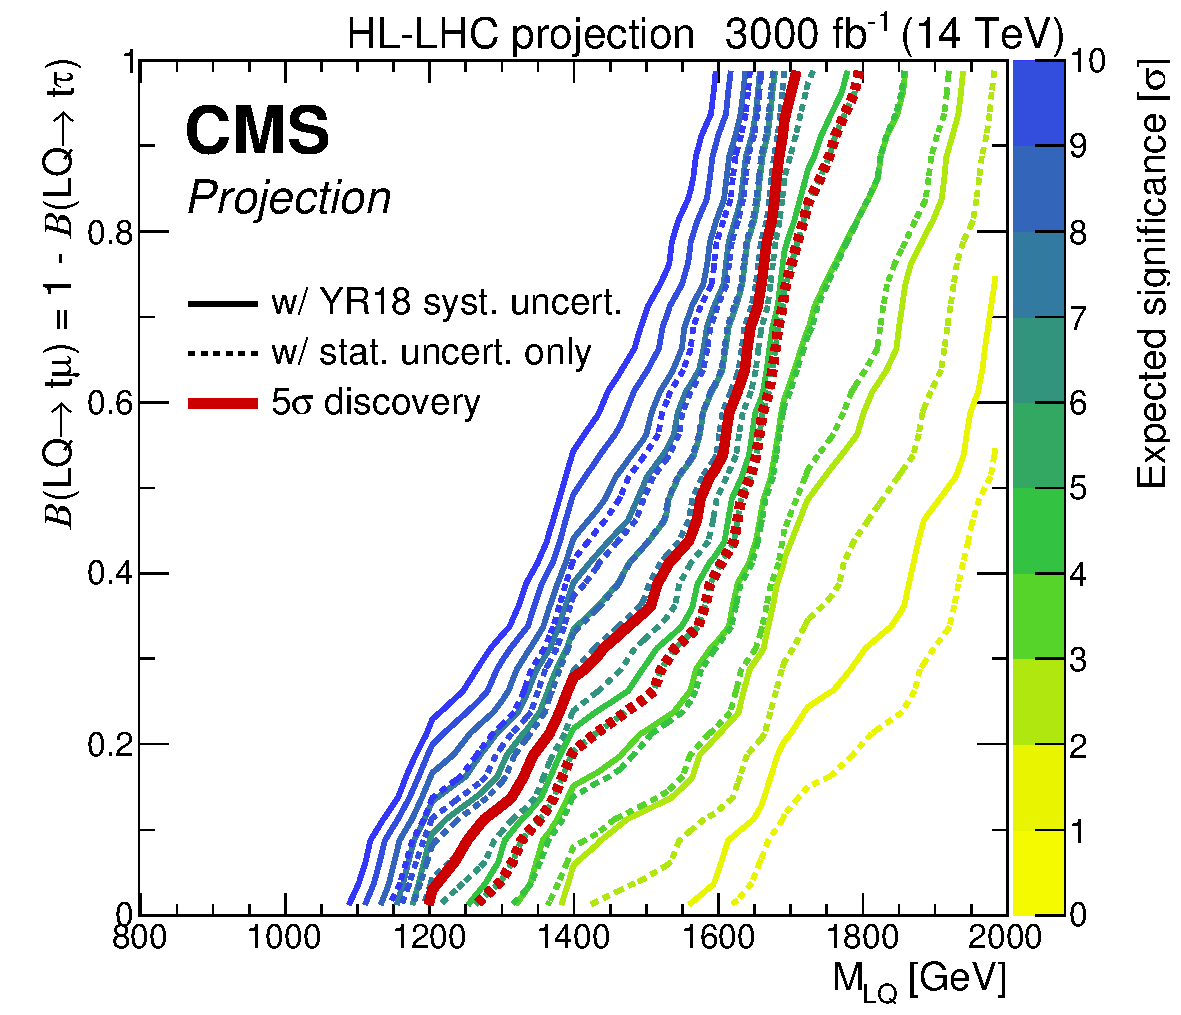
\includegraphics[width = 0.49\textwidth]{\main/section7OtherSignatures/img/LQpairs_Sign_2d.pdf}
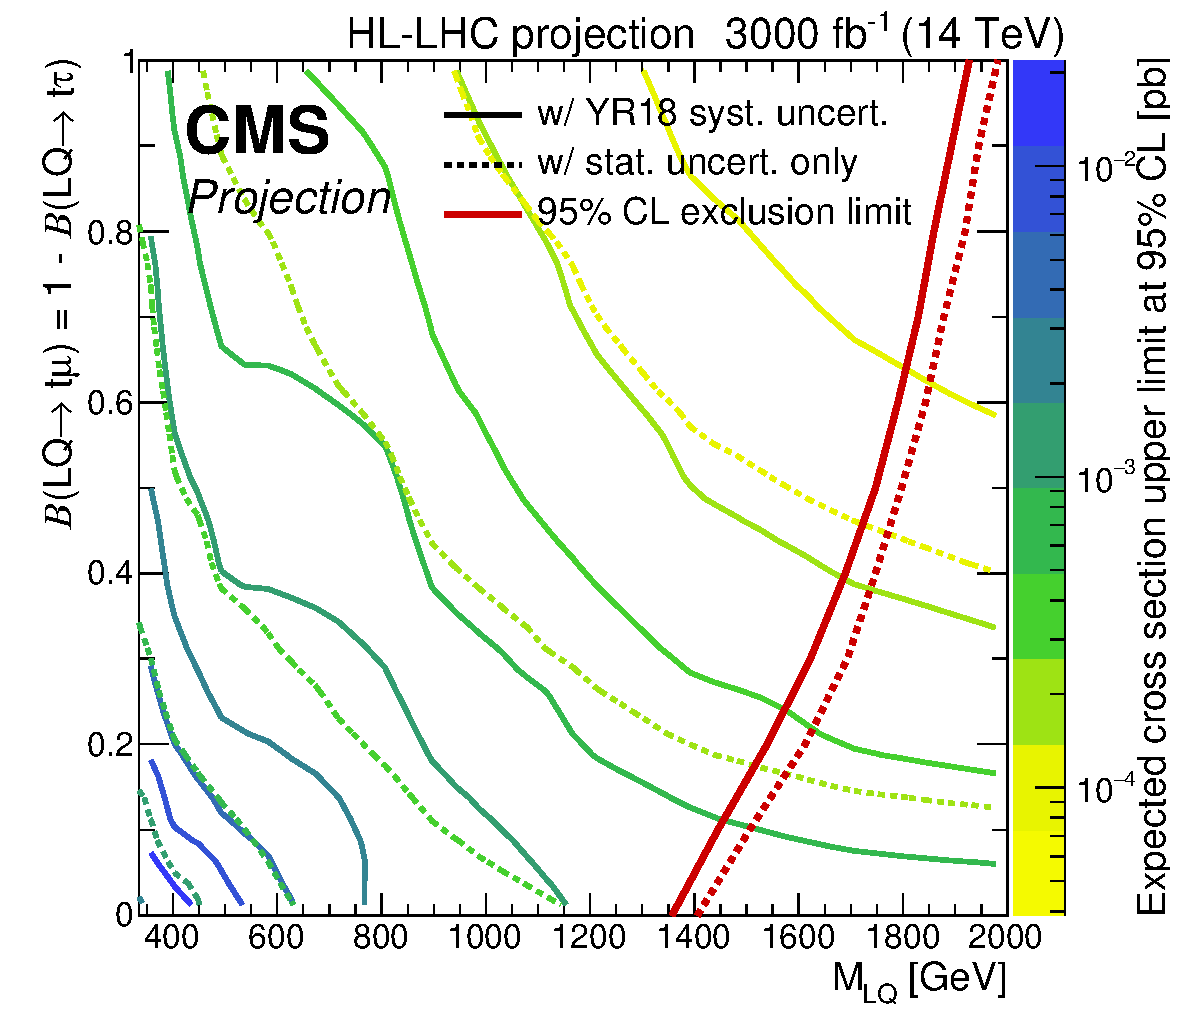
\includegraphics[width = 0.49\textwidth]{\main/section7OtherSignatures/img/LQpairs_Limits_2d.pdf}
\caption{Expected significances (left) and expected upper limits on the LQ pair-production cross section at the 95\%~\cl (right) as a function of the LQ mass and the branching fraction. Color-coded lines represent lines of a constant expected significance or cross section limit, respectively. The red lines indicate the 5$\sigma$ discovery level (left) and the mass exclusion limit (right).}
\label{fig:LQpairs:limits2d}
\end{figure}